% ----------------------------------------------------------
% Abordagem proposta 
% ----------------------------------------------------------
\chapter{Abordagem Proposta}
\label{chap:abordagem}
% ----------------------------------------------------------


No contexto de jogos digitais, treinar um agente para superar os jogadores humanos e otimizar sua pontuação pode nos ensinar como otimizar processos diferentes em uma variedade de subcampos intrigantes \cite{comi:teach:AI:DRL:2018}. Uma solução proposta na literatura, obtendo ótimos resultados, e que tem como objetivo treinar um computador pra aprender e desenvolver estratégias para jogar diferentes jogos, é o \textit{deep reinforcement learning} (DRL). 

No presente trabalho é proposto a implementação de uma inteligência artificial que, utilizando um algoritmo de \textit{deep reinforcement learning}, seja capaz de aprender a jogar diferentes jogos e desenvolver estratégias para maximizar sua pontuação.

Diante das peculiaridades e restrições do problema discutidos em \textbf{\ref{sec:descricao_do_problema}}, a biblioteca \textit{Allegro} foi escolhida como a base para a implementação dos jogos que serão apresentados ao sistema.
O \textit{Allegro} é uma biblioteca multiplataforma destinada principalmente a jogos de vídeo e programação multimídia. A biblioteca fornece rotinas de baixo nível comumente necessárias na programação de jogos, como a criação de janelas, aceitação de entrada do usuário, carregamento de dados, desenho de imagens, reprodução de sons etc \cite{allegro}.

Por fim, para auxiliar a implementação do sistema, será utilizado um \textit{Allegro Learning Enviroment}, uma ferramenta para o desenvolvimento de inteligência artificial em jogos implementados em \textit{Allegro}. Seu objetivo é oferecer uma plataforma que facilite o desenvolvimento de algoritmos de ML para jogos em \textit{Allegro}.



% section contextualização (end)
\section{\textit{Deep Learning}}


 O \textit{deep learning} (DL) é uma área do aprendizado de máquina que propõe que os computadores aprendam com a experiência, se ajustem à novas entradas de dados e compreendam o mundo em termos de hierarquia de conceitos, sendo cada conceito definido por sua relação com conceitos mais simples. 
 Ao reunir conhecimento a partir da experiência, essa abordagem evita a necessidade dos operadores humanos de especificar formalmente todo o conhecimento que o computador precisa. Além disso, a hierarquia de conceitos permite que o computador aprenda conceitos complexos, construindo-os a partir de conceitos mais simples. O \textit{deep learning} apresenta grande poder e flexibilidade a nos permitir o treinamento de computadores para cumprir tarefas específicas ao processar grandes quantidades de dados e reconhecer padrões nesses dados.


 A \textbf{Figura \ref{hierarquia-conceitos-dl}} mostra como um sitema de \textit{deep learning} representa o conceito de imagem de uma pessoa combinando conceitos mais simples, como cantos e contornos, que por sua vez são definidos em termos de arestas. 

 O mapeamento de funções de um conjunto de pixels para uma identidade de objeto é uma tarefa complicada. O algoritmo de \textit{deep learning} resolve essa dificuldade dividindo o mapeamento complicado desejado em séries de mapeamentos simples aninhados, cada um deles descrito por uma camada diferente do modelo. A entrada é apresentada na camada visível,
 em seguida, uma série de camadas ocultas extrai recursos cada vez mais abstratos da imagem. A camada de saída obtém a identidade de objeto abstrata a partir dos conceitos obtidos pelas camadas ocultas.


 \begin{figure}[h]
 \centering
 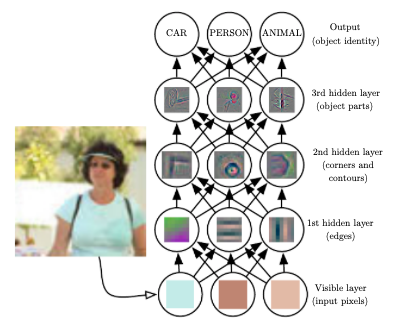
\includegraphics[width=.5 \textwidth]{conteudo/imgs/hierarquia-conceitos-dl.png}
 \caption[Ilustração de um modelo de aprendizado profundo]{Ilustração de um modelo de aprendizado profundo. Cada camada é capaz de identificar dados de complexidade crescente a partir dos pixels pasados para a camada de entrada. Imagem retirada de \cite{Goodfellow-et-al-2016}}
 \label{hierarquia-conceitos-dl}
 \end{figure}
 % \clearpage

 \section{\textit{Reinforcement Learning}} % (fold)
 \label{sec:reinforcement_learning}

 O aprendizado por reforço ou \textit{reinforcement learning} (RL) é uma abordagem computacional para entender e automatizar o aprendizado direcionado a objetivos e a tomada de decisões. O aprendizado por reforço distingue-se de outras abordagens computacionais por sua ênfase na aprendizagem de um agente apartir da interação direta com seu ambiente, sem exigir supervisão exemplar ou modelos completos do ambiente \cite{reinforcement-learning-intro-2018}.

 Em algoritmos de \textit{reinforcement learning}, o agente não é informado sobre quais ações executar, mas, em vez disso, deve descobrir quais ações geram mais recompensa, através de tentativa e erro. Em alguns casos mais interessantes, as ações podem afetar não apenas a recompensa imediata, mas também a próxima situação e, com isso, todas as recompensas subsequentes. Essas duas características - pesquisa por tentativa e erro e recompensa atrasada - são as duas características distintivas mais importantes do aprendizado por reforço.

 % O aprendizado por reforço é diferente do aprendizado supervisionado, o tipo de aprendizado estudado na maioria das pesquisas atuais no campo do aprendizado de máquina. Aprendizado supervisionado é aprender com um conjunto de treinamento de exemplos rotulados fornecidos por um supervisor externo qualificado. O objetivo desse tipo de aprendizado é o sistema extrapolar ou generalizar suas respostas para que ele atue corretamente em situações não presentes no conjunto de treinamento.
 %  % Este é um tipo importante de aprendizado, mas por si só não é adequado para aprender com a interação. Em problemas interativos, muitas vezes é impraticável obter exemplos do comportamento desejado que sejam corretos e representativos de todas as situações nas quais o agente precisa agir. Em um território desconhecido - onde se espera que a aprendizagem seja mais benéfica - um agente deve ser capaz de aprender com sua própria experiência.

 %  O aprendizado por reforço também é diferente do que os pesquisadores de aprendizado de máquina chamam de aprendizado não supervisionado, que geralmente consiste em encontrar estruturas ocultas em coleções de dados não rotulados. Os termos aprendizado supervisionado e aprendizado não supervisionado parecem classificar exaustivamente os paradigmas de aprendizado de máquina, mas não o fazem. Embora se possa ficar tentado a pensar no aprendizado por reforço como um tipo de aprendizado não supervisionado, porque não se baseia em exemplos de comportamento correto, o aprendizado por reforço está tentando maximizar um sinal de recompensa em vez de tentar encontrar uma estrutura oculta. Descobrir a estrutura na experiência de um agente certamente pode ser útil no aprendizado por reforço, mas por si só não aborda o problema do aprendizado por reforço de maximizar um sinal de recompensa. Portanto, o aprendizado por reforço é considerado como um terceiro paradigma de aprendizado de máquina, ao lado de aprendizado supervisionado, aprendizado não supervisionado e talvez outros paradigmas  \cite{reinforcement-learning-intro-2018}.

 Além do agente e do ambiente, é interessante ressaltar outros elementos importantes de um sistema de aprendizado por reforço: a \textbf{política}, o \textbf{sinal de recompensa} e a \textbf{função de valor}.

 A \textbf{política} define a maneira que o agente deve se comportar em um determinado momento. 
 Uma política é basicamente um mapeamento dos estados do ambiente para as ações a serem tomadas quando nesses estados. 
 A política em casos mais simples ter a forma de uma função simples ou uma tabela de pesquisa, enquanto em casos mais complexos pode envolver cálculos mais extensivos. 
 Em geral, as políticas podem ser estocásticas, especificando probabilidades para cada ação.

 Um \textbf{sinal de recompensa} define o objetivo de um problema de aprendizado por reforço. 
 Em cada etapa, o ambiente envia ao agente de aprendizado por reforço um único número que funciona como uma recompensa para o agente. 
 O único objetivo do agente é maximizar a recompensa total que recebe a longo prazo.
 O sinal de recompensa define, portanto, quais são os eventos bons e ruins para o agente. 
 O sinal de recompensa é a base principal para alterar a política - se uma ação selecionada pela política for seguida por uma baixa recompensa, a política poderá ser alterada para selecionar outra ação nessa situação no futuro. 
 Em geral, os sinais de recompensa podem ser funções estocásticas do estado do ambiente e das ações tomadas.

 Enquanto o sinal de recompensa indica o que é bom em um sentido imediato, uma \textbf{função de valor} especifica o que é bom a longo prazo. 
 O valor de um estado representa a quantidade total de recompensa que um agente pode esperar acumular no futuro, a partir desse estado. 
 Enquanto as recompensas determinam a conveniência imediata e intrínseca dos estados ambientais, os valores indicam a conveniência a longo prazo dos estados após levar em conta os estados que provavelmente seguirão e as recompensas disponíveis nesses estados. 
 Por exemplo, um estado sempre pode gerar uma recompensa imediata baixa, mas ainda tem um valor alto porque é seguido regularmente por outros estados que produzem recompensas altas. Ou o contrário poderia ser verdade. 

 A \textbf{Figura \ref{rl-diagram}} mostra um diagrama de aprendizagem por reforço relacionando o agente de aprendizado com o ambiente no qual ele é inserido.
 O ambiente representa o mundo pelo qual o agente se move. O ambiente nada mais é do que um sistema que toma o estado atual e a ação do agente como entrada e retorna como saída a recompensa do agente e seu próximo estado. 

 Ambientes podem ser modelados como funções que transformam uma ação executada no estado atual, no próximo estado e uma recompensa. Já os agentes podem ser modelados como funções que transformam o novo estado e recompensam na próxima ação. 
 Podemos conhecer a função do agente, mas não podemos conhecer a função do ambiente. É uma caixa preta onde só vemos as entradas e saídas. 
 % É como o relacionamento da maioria das pessoas com a tecnologia: sabemos o que faz, mas não sabemos como funciona. 
 O aprendizado por reforço representa a tentativa de um agente de aproximar a função do ambiente, para que possamos enviar ações para o ambiente de caixa preta que maximize as recompensas que ele distribui \cite{beg-guide-rl}.

 \begin{figure}[h]
  \centering
  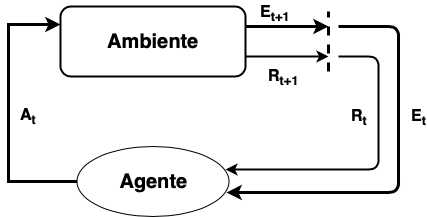
\includegraphics[width=.6 \textwidth]{conteudo/imgs/rl-diagram.png}
  \caption[Diagrama de aprendizagem por reforço]{Diagrama de aprendizagem por reforço. No \textit{loop} de \textit{feedback} acima, os subscritos indicam as etapas de tempo $t$ e $t + 1$, cada uma das quais se refere a estados diferentes: o estado no momento $t$ e o estado no momento $t + 1$. 
 % Diferente de outras formas de aprendizado de máquina - como aprendizado supervisionado e não supervisionado - o aprendizado por reforço só pode ser pensado sequencialmente em termos de pares de ação de estado que ocorrem um após o outro.
  A ação $A_t$ de um agente é determinada por sua \textbf{política}, que por sua vez é uma função que depende do estado atual do sistema $E_t$. A política de um agente tem como objetivo maximizar a \textbf{função de valor} que é calculada utilizando o \textbf{sinal de recompensa} $R_t$. O ambiente se comporta como um sistema caixa preta que transforma uma ação executada no estado atual $A_t$, no próximo estado $E_{t+1}$ e uma recompensa $R_{t+1}$
  }
  \label{rl-diagram}
 \end{figure}

 As escolhas de ação são feitas com base em julgamentos de valor.
 Buscamos ações que gerem estados de maior valor, e não de maior recompensa, porque essas ações obtêm a maior quantidade de recompensa a longo prazo. 
 % Infelizmente, é muito mais difícil determinar valores do que determinar recompensas. 
 As recompensas são basicamente dadas diretamente pelo ambiente, mas os valores devem ser estimados e re-estimados a partir das sequências de observações que um agente faz ao longo de toda a sua vida útil.


 O \textit{deep reinforcement learning} (DRL) é uma abordagem do \textit{deep learning} que, em contraste a abordagens mais tradicionais como o aprendizado supervisionado e não supervisionado, utiliza as técnicas de aprendizagem por reforço para treinar o agente. Essa abordagem consiste em fornecer ao sistema parâmetros relacionados ao seu estado e uma recompensa positiva ou negativa com base em suas ações. Nenhuma regra sobre o jogo é dada e, inicialmente, o agente não tem nenhuma informação sobre o que precisa fazer. O objetivo do sistema é descobrir e elaborar uma estratégia para maximizar sua pontuação - ou recompensa.



\section{Aplicação de DRL em um \textit{Allegro Learning Enviroment}} % (fold)
 \label{sec:allegro_learning_enviroment}

 O \textit{Arcade Learning Enviroment} é uma ferramenta de software que oferece uma interface para interagir com ambientes de jogos Atari 2600 emulados. Seu objetivo é oferecer uma plataforma que facilite o desenvolvimento de agentes de aprendizado para aprender a jogar jogos Atari. Essa ferramenta também fornece uma camada de manipulação de jogos que
 transforma cada jogo em um problema padrão de aprendizado por reforço, identificando a pontuação acumulada e se o jogo terminou. \cite{arcade-learning-enviroment}

 Inspirado na plataforma descrita acima, este trabalho visa a utilização de um \textit{Allegro Learning Enviroment}, que funcionaria de forma semelhante ao \textit{Arcade Learning Enviroment}, com a distinção de que o primeiro seria uma plataforma voltada para jogos implementados em \textit{Allegro}. O \textit{Allegro Learning Enviroment} (ALE) terá como base a ferramenta implementada por \cite{silva:amb-jd-allegro}, que oferece um ambiente facilitador ao estudo de soluções de IA aplicada em jogos. Essa ferramenta fornece funcionalidades como a exportação dos comandos básicos de um jogo, que precisam ser passados para o agente para que o mesmo tenha conhecimento dos limites físicos do ambiente no qual está inserido. Isso permite que o pesquisador não fique limitado a um jogo existente, mas possa usar qualquer jogo que ele tenha acesso ao código fonte e feito em \textit{Allegro}.

 Para o treinamento do agente, serão utilizados capturas da tela em cada estado do jogo, obtidas pelo ALE. A partir dessas imagens serão extraídas  as informações do estado atual do jogo (posição do jogador, obstáculos, etc), de forma a determinar qual a melhor ação do agente para a situação na qual ele se encontra. A utilização de capturas de tela como entradas para o agente permite que a IA seja treinada para situações em que hajam obstáculos gerados de forma aleatória. A partir dessas imagens, o agente deverá ser capaz de identificar tais obstáculos, sua localização e a melhor maneira de lidar com os mesmos.

 Em relação aos jogos nos quais o agente será treinado, a proposta é de se utilizar diferentes jogos de diferentes complexidades para avaliar o potencial do sistema. Os jogos serão obtidos de fontes de código aberto disponíveis \textit{online} ou, caso seja necessário, serão implementados com os requisitos necessário para o projeto.



 

 % [TODO]


 % \section{Modelagem matemática} % (fold)
 % \label{sec:modelagem_matemática}
 
 % section modelagem_matemática (end)




